% 第 2 章 数据结构与算法
\renewcommand{\codeInset}{63bp}
上一章中，我们为栈和队列这两个抽象数据类型创建了类。本章我们将继续处理列表和集合这两个抽象数据类型。

与上一章的栈和队列类似，列表（list）是一种有头有尾的有序结构。不过，列表允许在任意位置加入和移除值，还可以遍历列表。

而集合（set）则是一种由值组成的无序结构。对于集合，我们唯一能说的是某个值是否存在；我们无法说出某个值相对于其他任何值的位置关系。

本章将涵盖以下主题：

\begin{itemize}
\item 我们先实现相当简单但低效的列表类和集合类，并研究搜索与排序的基础算法。
\item 然后创建更高级版本的列表类和集合类，研究更高级的搜索与排序算法。我们还会引入一些新概念，如模板、运算符重载、异常和引用重载。
\item 我们还将研究线性搜索（linear search）和二分搜索（binary search）这两种搜索算法：前者可用于任何序列（无论有序还是无序），但效率较低；后者效率更高，但只能用于有序序列。
\item 最后，我们将研究插入排序（insert sort）、选择排序（select sort）和冒泡排序（bubble sort）这些相当简单的排序算法，以及更高级、更高效的归并排序（merge sort）和快速排序（quick sort）算法。
\end{itemize}

\section{列表类}

链表类比栈和队列更复杂，是一种更复杂的抽象数据类型。我们可以在列表的任意位置加入和移除值，也可以遍历列表。

\subsection{Cell 类}

本节的单元格是栈和队列两节中单元格的扩展。与它们类似，单元格存放一个值和一个指向下一个单元格的指针；不过，这个版本还持有一个指向前一个单元格的指针，这使得本节的链表成为双向链表（double-linked list）。

注意，这里的构造函数是 private 的，这意味着单元格对象只能由它自己的成员函数创建。不过，有一种办法可以绕过这一限制：我们可以把某个类或函数定义为 LinkedList 的友元（friend）。这里，我们把 LinkedList 定义为 Cell 的友元，也就是说，LinkedList 可以访问 Cell 的所有 private 和 protected 成员——包括构造函数——从而可以创建 Cell 对象。

\medskip\noindent{\ttfamily\bfseries Cell.h}

\begin{codebox}
class Cell {
  private:
    Cell(double value, Cell *previous, Cell *next);
    friend class LinkedList;

  public:
    double getValue() const { return m_value; }
    void setValue(double value) { m_value = value; }

    Cell *getPrevious() const { return m_previous; }
    void setPrevious(Cell *previous) { m_previous = previous; }

    Cell *getNext() const { return m_next; }
    void setNext(Cell *getNext) { m_next = getNext; }

  private:
    double m_value;
    Cell *m_previous, *m_next;
};
\end{codebox}

\medskip\noindent{\ttfamily\bfseries Cell.cpp}

\begin{codebox}
#include "Cell.h"

Cell::Cell(double value, Cell *previous, Cell *next)
 :m_value(value),
  m_previous(previous),
  m_next(next) {
  // Empty.
}
\end{codebox}

\subsection{Iterator 类}

遍历列表时，我们需要一个迭代器（iterator），它被初始化为列表的开头，然后一步一步地移向列表末尾。与前面的单元格类似，Iterator 的构造函数也是 private 的，不过我们同样把 LinkedList 定义为 Iterator 的友元。

\medskip\noindent{\ttfamily\bfseries Iterator.h}

\begin{codebox}
class Iterator {
  private:
    Iterator(Cell *cellPtr);
    friend class LinkedList;

  public:
    Iterator();
\end{codebox}

第三个构造函数是复制构造函数（copy constructor）。它接受另一个迭代器并复制它。我们不能直接接受迭代器对象作为参数，而是要定义一个引用参数。\& 符号表明该参数是对迭代器对象的引用，而不是迭代器对象本身。这样，传递给参数的是迭代器的内存地址，而不是对象本身。我们还声明被引用的对象为常量，这样它就不会被构造函数修改。

在本例中必须使用引用参数。如果参数只是一个简单的迭代器对象，就会造成无限循环的初始化。而在其他情况下，我们出于效率的考虑使用这一技巧：传递对象的地址比把对象本身复制为参数更省时间、更省内存：

\begin{codebox}
    Iterator(const Iterator& iterator);

    double getValue() { return m_cellPtr->getValue(); }
    void setValue(double value) { m_cellPtr->setValue(value); }
\end{codebox}

hasNext 方法在迭代器尚未到达列表末尾时返回 true，而 next 方法把迭代器向列表末尾方向前移一步，如下例所示：

\begin{codebox}
    bool hasNext() const { return (m_cellPtr != nullptr); }
    void next() { m_cellPtr = m_cellPtr->getNext(); }
\end{codebox}

同样，hasPrevious 方法在迭代器尚未到达列表开头时返回 true，而 previous 方法把迭代器向列表开头方向后退一步：

\begin{codebox}
    bool hasPrevious() const { return (m_cellPtr != nullptr); }
    void previous() { m_cellPtr = m_cellPtr->getPrevious(); }

  private:
    Cell *m_cellPtr;
};
\end{codebox}

\medskip\noindent{\ttfamily\bfseries Iterator.cpp}

\begin{codebox}
#include "Cell.h"
#include "Iterator.h"

Iterator::Iterator(Cell *cellPtr)
 :m_cellPtr(cellPtr) {
  // Empty.
}

Iterator::Iterator()
 :m_cellPtr(nullptr) {
  // Empty.
}

Iterator::Iterator(const Iterator& iterator)
 :m_cellPtr(iterator.m_cellPtr) {
  // Empty.
}
\end{codebox}

\subsection{LinkedList 类}

LinkedList 类持有查找、加入、插入和移除值的方法，以及比较列表的方法。此外，它还持有读取和写出列表的方法，以及正向和反向遍历列表的方法。这个链表实际上是一个双向链表：我们可以沿着单元格之间的链接双向移动——既可以从头走到尾，也可以从尾走回头。

\medskip\noindent{\ttfamily\bfseries LinkedList.h}

\begin{codebox}
class LinkedList {
  public:
    LinkedList();
\end{codebox}

复制构造函数和 assign 方法都会复制给定的列表：

\begin{codebox}
    LinkedList(const LinkedList& list);
    void assign(const LinkedList& list);
\end{codebox}

析构函数释放为链表中各个单元格分配的所有内存：

\begin{codebox}
    ~LinkedList();

    int size() const {return m_size;}
    bool empty() const {return (m_size == 0);}
\end{codebox}

find 方法搜索某个值。如果找到了该值，就返回 true，并把 findIterator 设置为该值所在的位置：

\begin{codebox}
    bool find(double value, Iterator& findIterator);
\end{codebox}

equal 和 notEqual 方法把当前链表与给定链表进行比较，分别在相等或不相等时返回 true，如下面的代码片段所示：

\begin{codebox}
    bool equal(const LinkedList& list) const;
    bool notEqual(const LinkedList& list) const;
\end{codebox}

如果我们想把一个值或另一个列表加入现有列表，该怎么办？add 方法把一个值或另一个列表加到当前列表的末尾，而 insert 则把一个值或一个列表插入到迭代器给出的位置：

\begin{codebox}
    void add(double value);
    void add(const LinkedList& list);

    void insert(const Iterator& insertPosition, double value);

    void insert(const Iterator& insertPosition,
                const LinkedList& list);
\end{codebox}

erase 方法删除给定位置上的值，而 clear 删除列表中的每一个值，如下例所示：

\begin{codebox}
    void erase(const Iterator& erasePosition);
    void clear();
\end{codebox}

remove 方法把从第一个迭代器到最后一个迭代器（含两端）之间的值都移除。第二个参数是默认参数，意思是这个方法既可以用一个参数调用，也可以用两个参数调用。在只用一个参数的情况下，第二个参数取声明中给出的值——这里是 Iterator(nullptr)，它表示列表末尾之后一步的位置。这意味着当只用一个迭代器调用 remove 时，从该迭代器（含）到列表末尾的所有值都会被移除。nullptr 指针实际上是一种特殊的指针，它会被转换成它所指向或所比较的类型——这里是 Cell 指针。通俗地说，如果一个指针的值是 nullptr，我们就说这个指针是空的：

\begin{codebox}
    void remove(const Iterator& firstPosition,
                const Iterator& lastPosition = Iterator(nullptr));
\end{codebox}

first 和 last 方法返回位于列表第一个值和最后一个值处的迭代器：

\begin{codebox}
    Iterator first() const { return Iterator(m_firstCellPtr); }
    Iterator last() const { return Iterator(m_lastCellPtr); }
\end{codebox}

read 和 write 方法从输入文件流中读取列表的值，并把列表的值写到输出文件流。文件流用来与文件进行通信。注意，我们前面几节用过的 cin 和 cout 对象实际上就是输入流和输出流对象：

\begin{codebox}
    void read(istream& inStream);
    void write(ostream& outStream);
\end{codebox}

与前面一节的队列类似，列表持有指向链表中第一个和最后一个单元格的指针：

\begin{codebox}
  private:
    int m_size;
    Cell *m_firstCellPtr, *m_lastCellPtr;
};
\end{codebox}

\medskip\noindent{\ttfamily\bfseries LinkedList.cpp}

\begin{codebox}
#include <IOStream>
using namespace std;

#include "Cell.h"
#include "Iterator.h"
#include "List.h"

LinkedList::LinkedList()
 :m_size(0),
  m_firstCellPtr(nullptr),
  m_lastCellPtr(nullptr) {
  // Empty.
}
\end{codebox}

复制构造函数只是调用 assign 来复制列表参数的值：

\begin{codebox}
LinkedList::LinkedList(const LinkedList& list) {
  assign(list);
}
\end{codebox}

assign 方法把给定的列表复制到自己的链表中：

\begin{codebox}
void LinkedList::assign(const LinkedList& list) {
  m_size = 0;
  m_firstCellPtr = nullptr;
  m_lastCellPtr = nullptr;
  Cell *listCellPtr = list.m_firstCellPtr;
  add(list);
}
\end{codebox}

析构函数只是调用 clear，释放链表中各单元格所占用的所有内存：

\begin{codebox}
LinkedList::~LinkedList() {
  clear();
}
\end{codebox}

clear 方法遍历链表并释放每一个单元格：

\begin{codebox}
void LinkedList::clear() {
  Cell *currCellPtr = m_firstCellPtr;
\end{codebox}

对链表中的每个单元格，我们必须先把它的地址保存在 deleteCellPtr 中，在链表中向前移动一格，然后释放该单元格。如果直接对 currCellPtr 调用 delete，后面紧接的 getNext 调用就无法工作，因为那样我们就是在对一个已释放的对象调用方法：

\begin{codebox}
  while (currCellPtr != nullptr) {
    Cell *deleteCellPtr = currCellPtr;
    currCellPtr = currCellPtr->getNext();
    delete deleteCellPtr;
  }
\end{codebox}

当列表变空之后，两个单元格指针都为空，大小为零：

\begin{codebox}
  m_firstCellPtr = nullptr;
  m_lastCellPtr = nullptr;
  m_size = 0;
}
\end{codebox}

find 方法遍历链表，设置 findIterator，并在找到该值时返回 true。如果没有找到，就返回 false，findIterator 保持不变。为了让这一点成立，findIterator 必须是对 Iterator 对象的引用，而不是 Iterator 对象本身。用指向 Iterator 对象的指针也可以：

\begin{codebox}
bool LinkedList::find(double value, Iterator& findIterator) {
  Iterator iterator = first();

  while (iterator.hasNext()) {
    if (value == iterator.getValue()) {
      findIterator = iterator;
      return true;
    }

    iterator.next();
  }

  return false;
}
\end{codebox}

如果两个列表的大小不同，它们就不相等。同样，如果大小相同但值不同，它们也不相等：

\begin{codebox}
bool LinkedList::equal(const LinkedList& list) const {
  if (m_size != list.m_size) {
    return false;
  }

  Iterator thisIterator = first(), listIterator = list.first();

  while (thisIterator.hasNext()) {
    if (thisIterator.getValue() != listIterator.getValue()) {
      return false;
    }

    thisIterator.next();
    listIterator.next();
  }
\end{codebox}

不过，如果两个列表大小相同、值也相同，它们就相等：

\begin{codebox}
  return true;
}
\end{codebox}

在判断两个列表是否不相等时，我们只需调用 equal。感叹号（\texttt{!}）是逻辑非运算符，如下例所示：

\begin{codebox}
bool LinkedList::notEqual(const LinkedList& list) const {
  return !equal(list);
}
\end{codebox}

向列表加入值时，我们动态分配一个单元格：

\begin{codebox}
void LinkedList::add(double value) {
  Cell *newCellPtr = new Cell(value, m_lastCellPtr, nullptr);
\end{codebox}

如果第一个单元格指针为空，由于列表是空的，我们把它设置为指向新单元格：

\begin{codebox}
  if (m_firstCellPtr == nullptr) {
    m_firstCellPtr = newCellPtr;
  }
\end{codebox}

不过，如果第一个单元格指针不为空，说明列表非空，这时我们把最后一个单元格指针的 next 指针设置为指向新单元格：

\begin{codebox}
  else {
    m_lastCellPtr->setNext(newCellPtr);
  }
\end{codebox}

无论哪种情况，我们都把最后一个单元格指针设置为指向新单元格，并让列表的大小加一：

\begin{codebox}
  m_lastCellPtr = newCellPtr;
  ++m_size;
}
\end{codebox}

\subsection{向已有列表加入列表}

把整个列表加入列表时，对列表中的每一个值，我们都采取与前面 add 方法加入单个值时相同的做法：动态分配一个新单元格；如果第一个单元格指针为空，就让它指向新单元格；如果不为空，就把最后一个单元格指针的 next 指针设置为指向新单元格。无论哪种情况，最后都把最后一个单元格指针设置为指向新单元格：

\medskip\noindent{\ttfamily\bfseries LinkedList.cpp}

\begin{codebox}
void LinkedList::add(const LinkedList& list) {
  Cell *listCellPtr = list.m_firstCellPtr;
\end{codebox}

while 语句在条件为真期间不断重复执行。这里也就是在我们尚未到达列表末尾期间不断重复：

\begin{codebox}
  while (listCellPtr != nullptr) {
    double value = listCellPtr->getValue();
    Cell *newCellPtr = new Cell(value, m_lastCellPtr, nullptr);
\end{codebox}

如果 m\_firstCellPtr 为空，说明我们的链表还是空的，newCellPtr 指向新链表的第一个单元格。这时我们让 m\_firstCellPtr 指向新单元格：

\begin{codebox}
    if (m_firstCellPtr == nullptr) {
      m_firstCellPtr = newCellPtr;
    }
\end{codebox}

如果 m\_firstCellPtr 不为空，说明列表非空，此时不能修改 m\_firstCellPtr，而是把 m\_lastCellPtr 的 next 指针设置为指向新单元格：

\begin{codebox}
    else {
      m_lastCellPtr->setNext(newCellPtr);
    }
\end{codebox}

无论哪种情况，最后一个单元格指针都被设置为新单元格指针：

\begin{codebox}
    m_lastCellPtr = newCellPtr;
\end{codebox}

最后，列表单元格指针被设置为指向它的下一个单元格。最终这个指针会变成空，while 语句随之结束：

\begin{codebox}
    listCellPtr = listCellPtr->getNext();
  }

  m_size += list.m_size;
}
\end{codebox}

在迭代器给出的位置插入值时，我们把它的 previous 指针设置为指向列表中该位置之前的单元格（如果该位置是列表中的第一个，则为空）。然后，我们按照前面 add 方法中相同的方式检查第一个单元格指针是否为空：

\begin{codebox}
void LinkedList::insert(const Iterator& insertPosition,
                        double value) {
  Cell *insertCellPtr = insertPosition.m_cellPtr;
  Cell *newCellPtr =
    new Cell(value, insertCellPtr->getPrevious(), insertCellPtr);
  insertCellPtr->setPrevious(newCellPtr);

  if (insertCellPtr == m_firstCellPtr) {
    m_firstCellPtr = newCellPtr;
  }
  else {
    newCellPtr->getPrevious()->setNext(newCellPtr);
  }

  ++m_size;
}
\end{codebox}

插入整个列表时，我们首先检查该位置是否表示空指针。如果是，说明这个位置已经越过我们列表的末尾，这时直接改用 add：

\begin{codebox}
void LinkedList::insert(const Iterator& insertPosition,
                        const LinkedList& list) {
  Cell *insertCellPtr = insertPosition.m_cellPtr;

  if (insertCellPtr == nullptr) {
    add(list);
  }
  else {
    Cell *firstInsertCellPtr = nullptr,
         *lastInsertCellPtr = nullptr,
         *listCellPtr = list.m_firstCellPtr;

    while (listCellPtr != nullptr) {
      Cell *newCellPtr = new Cell(listCellPtr->getValue(),
                                  lastInsertCellPtr, nullptr);

      if (firstInsertCellPtr == nullptr) {
        firstInsertCellPtr = newCellPtr;
      }
      else {
        lastInsertCellPtr->setNext(newCellPtr);
      }

      lastInsertCellPtr = newCellPtr;
      listCellPtr = listCellPtr->getNext();
    }
\end{codebox}

我们把 firstInsertCellPtr 与 nullptr 进行比较，检查待插入的列表是否为空。由于 firstInsertCellPtr 指向列表的第一个值，它为空就意味着列表为空：

\begin{codebox}
    if (firstInsertCellPtr != nullptr) {
      if (insertCellPtr->getPrevious() != nullptr) {
        insertCellPtr->getPrevious()->setNext(firstInsertCellPtr);
        firstInsertCellPtr->
          setPrevious(insertCellPtr->getPrevious());
      }
      else {
        m_firstCellPtr = firstInsertCellPtr;
      }
    }

    if (lastInsertCellPtr != nullptr) {
      lastInsertCellPtr->setNext(insertCellPtr);
      insertCellPtr->setPrevious(lastInsertCellPtr);
    }

    m_size += list.m_size;
  }
}
\end{codebox}

\subsection{从列表中删除值}

erase 方法只是调用 remove，把给定位置同时作为起始和结束位置：

\begin{codebox}
void LinkedList::erase(const Iterator& removePosition) {
  remove(removePosition, removePosition);
}
\end{codebox}

从列表中删除值时，我们遍历列表，并为每一个要移除的值释放其单元格：

\begin{codebox}
void LinkedList::remove(const Iterator& firstPosition,
           const Iterator& lastPosition /*= Iterator(nullptr)*/) {
  Cell *firstCellPtr = firstPosition.m_cellPtr,
       *lastCellPtr = lastPosition.m_cellPtr;
  lastCellPtr = (lastCellPtr == nullptr)
                ? m_lastCellPtr : lastCellPtr;

  Cell *previousCellPtr = firstCellPtr->getPrevious(),
       *nextCellPtr = lastCellPtr->getNext();

  Cell *currCellPtr = firstCellPtr;
  while (currCellPtr != nextCellPtr) {
    Cell *deleteCellPtr = currCellPtr;
    currCellPtr = currCellPtr->getNext();
    delete deleteCellPtr;
    --m_size;
  }
\end{codebox}

删除这些单元格时有三种情况要考虑。如果第一个被删除单元格之前的最后一个单元格不为空——意思是删除位置之前还有列表的剩余部分——我们就把它的 next 指针设置为指向删除位置之后的第一个单元格。如果第一个被删除单元格之前的最后一个单元格为空，我们就把第一个单元格指针设置为指向删除位置之后的那个单元格：

\begin{codebox}
  if (previousCellPtr != nullptr) {
    previousCellPtr->setNext(nextCellPtr);
  }
  else {
    m_firstCellPtr = nextCellPtr;
  }
\end{codebox}

对于最后一个被删除单元格之后的列表剩余位置，我们也做同样的事情。如果删除部分之后还有列表的剩余部分，我们就把它的第一个单元格的 previous 指针设置为指向删除部分之前剩余列表的最后一个单元格：

\begin{codebox}
  if (nextCellPtr != nullptr) {
    nextCellPtr->setPrevious(previousCellPtr);
  }
  else {
    m_lastCellPtr = previousCellPtr;
  }
}
\end{codebox}

读取列表时，我们先读取列表的大小，然后再读取各个值：

\begin{codebox}
void LinkedList::read(istream& inStream) {
  int size;
  inStream >> size;

  int count = 0;
  while (count < size) {
    double value;
    inStream >> value;
    add(value);
    ++count;
  }
}
\end{codebox}

写出列表时，我们把各个值用逗号分隔、用方括号（\texttt{"["} 与 \texttt{"]"}）括起来写出：

\begin{codebox}
void LinkedList::write(ostream& outStream) {
  outStream << "[";
  bool firstValue = true;

  Iterator iterator = first();
  while (iterator.hasNext()) {
    outStream << (firstValue ? "" : ",") << iterator.getValue();
    firstValue = false;
    iterator.next();
  }

  outStream << "]";
}
\end{codebox}

我们向列表加入一些值来测试它，然后再正向、反向遍历这些值。

\medskip\noindent{\ttfamily\bfseries Main.cpp}

\begin{codebox}
#include <IOStream>
using namespace std;

#include "Cell.h"
#include "Iterator.h"
#include "List.h"

void main() {
  LinkedList list;
  list.add(1);
  list.add(2);
  list.add(3);
  list.add(4);
  list.add(5);
  list.write(cout);
  cout << endl;

  { Iterator iterator = list.first();
    while (iterator.hasNext()) {
      cout << iterator.getValue() << " ";
      iterator.next();
    }
    cout << endl;
  }

  { Iterator iterator = list.last();
    while (iterator.hasPrevious()) {
      cout << iterator.getValue() << " ";
      iterator.previous();
    }
    cout << endl;
  }
}
\end{codebox}

执行代码后，输出显示在一个命令窗口中：

\begin{center}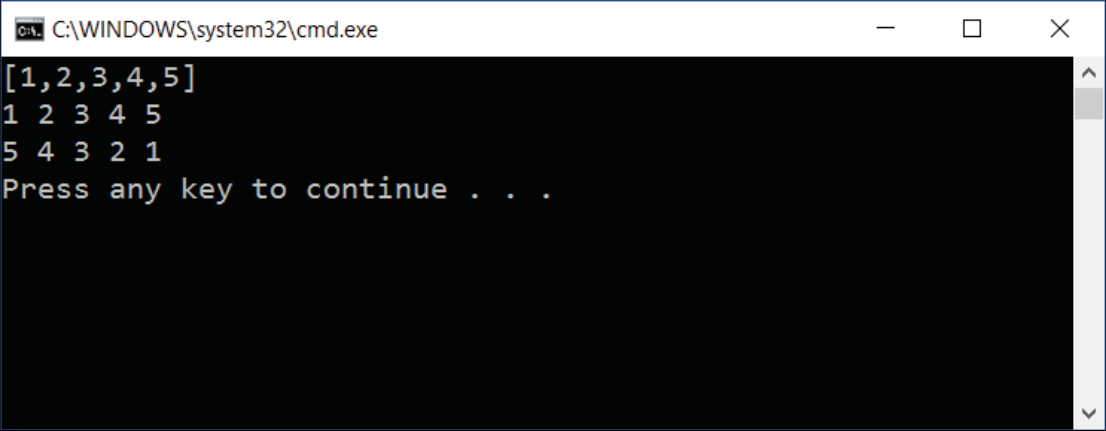
\includegraphics[width=0.72\textwidth]{images/p064_i05.png}\end{center}

\section{集合类}

集合是一种没有重复元素的无序结构。Set 类是 LinkedList 的子类。注意这里的继承方式是 private 的，这使得 LinkedList 的所有 public 和 protected 成员在 Set 中都变成 private。

\medskip\noindent{\ttfamily\bfseries Set.h}

\begin{codebox}
class Set : private LinkedList {
  public:
    Set();
    Set(double value);
    Set(const Set& set);
    void assign(const Set& set);
    ~Set();
\end{codebox}

equal 方法在集合拥有这些值时返回 true。注意，我们并不关心集合中值的任何顺序：

\begin{codebox}
    bool equal(const Set& set) const;
    bool notEqual(const Set& set) const;
\end{codebox}

exists 方法分别在给定值存在、或给定集合中每个值都存在时返回 true：

\begin{codebox}
    bool exists(double value) const;
    bool exists(const Set& set) const;
\end{codebox}

insert 方法插入给定值，或给定集合中的每个值。它只插入集合中尚不存在的值，因为集合不允许重复：

\begin{codebox}
    bool insert(double value);
    bool insert(const Set& set);
\end{codebox}

remove 方法在存在的情况下移除给定值，或给定集合中的每个值：

\begin{codebox}
    bool remove(double value);
    bool remove(const Set& set);
\end{codebox}

size、empty 和 first 方法只是调用 LinkedList 中的对应方法。由于集合没有顺序，再去覆盖 LinkedList 中的 end 方法就没有意义了：

\begin{codebox}
    int size() const { return LinkedList::size(); }
    bool empty() const { return LinkedList::empty(); }
    Iterator first() const { return LinkedList::first(); }
\end{codebox}

自由函数 unionSet、intersection 和 difference 是 Set 的友元，这意味着它们可以访问 Set 的所有 private 和 protected 成员。

\begin{myNotic}{p065_i00}{我们不能把 unionSet 方法命名为 union，因为 union 是 C++ 的关键字。}
\end{myNotic}

注意，当一个类中的方法被标记为友元时，它实际上并不是这个类的方法，而是一个函数：

\begin{codebox}
    friend Set unionSet(const Set& leftSet, const Set& rightSet);
    friend Set intersection(const Set& leftSet,
                            const Set& rightSet);
    friend Set difference(const Set& leftSet,
                          const Set& rightSet);
\end{codebox}

read 和 write 方法以与 LinkedList 中对应方法相同的方式读取和写出集合：

\begin{codebox}
    void read(istream& inStream);
    void write(ostream& outStream);
};
\end{codebox}

作为 Set 友元的 unionSet、intersection 和 difference 函数在类定义之外声明：

\begin{codebox}
Set unionSet(const Set& leftSet, const Set& rightSet);
Set intersection(const Set& leftSet, const Set& rightSet);
Set difference(const Set& leftSet, const Set& rightSet);
\end{codebox}

\medskip\noindent{\ttfamily\bfseries Set.cpp}

\begin{codebox}
#include <IOStream>
using namespace std;

#include "..\ListBasic\Cell.h"
#include "..\ListBasic\Iterator.h"
#include "..\ListBasic\List.h"
#include "Set.h"
\end{codebox}

构造函数调用 LinkedList 中的对应版本。实际上，默认构造函数（不带参数的那个）会隐式调用 LinkedList 的默认构造函数：

\begin{codebox}
Set::Set() {
  // Empty.
}

Set::Set(double value) {
  add(value);
}

Set::Set(const Set& set)
 :LinkedList(set) {
  // Empty.
}
\end{codebox}

析构函数隐式调用 LinkedList 中的对应版本，释放与集合中各值相关联的内存。在这里，我们其实可以省略析构函数，LinkedList 的析构函数照样会被调用——代码如下：

\begin{codebox}
Set::~Set() {
  // Empty.
}
\end{codebox}

assign 方法只是清空集合，然后加入给定的集合：

\begin{codebox}
void Set::assign(const Set& set) {
  clear();
  add(set);
}
\end{codebox}

如果两个集合大小相同，并且其中一个集合的每个值都存在于另一个集合中，那么这两个集合相等。这种情况下，另一个集合的每个值也必然存在于第一个集合中：

\begin{codebox}
bool Set::equal(const Set& set) const {
  if (size() != set.size()) {
    return false;
  }

  Iterator iterator = first();
  while (iterator.hasNext()) {
    if (!set.exists(iterator.getValue())) {
      return false;
    }

    iterator.next();
  }
  return true;
}

bool Set::notEqual(const Set& set) const {
  return !equal(set);
}
\end{codebox}

exists 方法使用 LinkedList 的迭代器遍历集合。如果找到该值，就返回 true：

\begin{codebox}
bool Set::exists(double value) const {
  Iterator iterator = first();

  while (iterator.hasNext()) {
    if (value == iterator.getValue()) {
      return true;
    }

    iterator.next();
  }

  return false;
}
\end{codebox}

第二个 exists 方法遍历给定的集合，只要其中有一个值在当前集合中不存在就返回 false；如果所有值都存在，则返回 true：

\begin{codebox}
bool Set::exists(const Set& set) const {
  Iterator iterator = set.first();

  while (iterator.hasNext()) {
    if (!exists(iterator.getValue())) {
      return false;
    }

    iterator.next();
  }

  return true;
}
\end{codebox}

第一个 insert 方法在值尚不存在于集合中时把它加入：

\begin{codebox}
bool Set::insert(double value) {
  if (!exists(value)) {
    add(value);
    return true;
  }

  return false;
}
\end{codebox}

第二个 insert 方法遍历给定的集合，通过调用第一个 insert 方法来插入每个值。这样，集合中尚不存在的每个值都会被插入：

\begin{codebox}
bool Set::insert(const Set& set) {
  bool inserted = false;
  Iterator iterator = set.first();

  while (iterator.hasNext()) {
    double value = iterator.getValue();

    if (insert(value)) {
      inserted = true;
    }

    iterator.next();
  }

  return inserted;
}
\end{codebox}

第一个 remove 方法在值存在于集合中时将其移除并返回 true；如果值不存在，则返回 false：

\begin{codebox}
bool Set::remove(double value) {
  Iterator iterator;
  if (find(value, iterator)) {
    erase(iterator);
    return true;
  }

  return false;
}
\end{codebox}

第二个 remove 方法遍历给定的集合并移除其中每一个值。只要至少移除了一个值，就返回 true：

\begin{codebox}
bool Set::remove(const Set& set) {
  bool removed = false;
  Iterator iterator = set.first();

  while (iterator.hasNext()) {
    double value = iterator.getValue();

    if (remove(value)) {
      removed = true;
    }

    iterator.next();
  }

  return removed;
}
\end{codebox}

\subsection{并集、交集与差集运算}

unionSet 函数创建一个以左侧集合初始化的结果集合，然后把右侧集合加入其中：

\begin{codebox}
Set unionSet(const Set& leftSet, const Set& rightSet) {
  Set result(leftSet);
  result.insert(rightSet);
  return result;
}
\end{codebox}

交集方法比并集或差集方法稍微复杂一些。两个集合 A 与 B 的交集可以定义为它们的并集与它们的差集之差：

$A \cap B = (A \cup B) - ((A - B) - (B - A))$

\begin{codebox}
Set intersection(const Set& leftSet, const Set& rightSet) {
  return difference(difference(unionSet(leftSet, rightSet),
                               difference(leftSet, rightSet)),
                    difference(rightSet, leftSet));
}
\end{codebox}

差集方法用左侧集合创建一个结果集合，然后从中移除右侧集合：

\begin{codebox}
Set difference(const Set& leftSet, const Set& rightSet) {
  Set result(leftSet);
  result.remove(rightSet);
  return result;
}
\end{codebox}

read 方法与 LinkedList 中的对应方法类似，不过这里调用的是 insert 而不是 add。这样，集合中就不会插入重复的值：

\begin{codebox}
void Set::read(istream& inStream) {
  int size;
  inStream >> size;

  int count = 0;
  while (count < size) {
    double value;
    inStream >> value;
    insert(value);
    ++count;
  }
}
\end{codebox}

write 方法也与 LinkedList 中的对应方法类似，不过这里集合用花括号（\texttt{"\{} 和 \texttt{"\}}）而不是方括号（\texttt{"[} 和 \texttt{"]"}）括起来：

\begin{codebox}
void Set::write(ostream& outStream) {
  outStream << "{";
  bool firstValue = true;
  Iterator iterator = first();

  while (iterator.hasNext()) {
    outStream << (firstValue ? "" : ",") << iterator.getValue();
    firstValue = false;
    iterator.next();
  }

  outStream << "}";
}
\end{codebox}

我们让用户输入两个集合，然后求出它们的并集、交集与差集，以此来测试集合。

\medskip\noindent{\ttfamily\bfseries Main.cpp}

\begin{codebox}
#include <IOStream>
using namespace std;

#include "..\ListBasic\Cell.h"
#include "..\ListBasic\Iterator.h"
#include "..\ListBasic\List.h"
#include "Set.h"

void main() {
  Set s, t;
  s.read(cin);
  t.read(cin);

  cout << endl << "s = ";
  s.write(cout);
  cout << endl;

  cout << endl << "t = ";
  t.write(cout);
  cout << endl << endl;

  cout << "union: ";
  unionSet(s, t).write(cout);
  cout << endl;

  cout << "intersection: ";
  unionSet(s, t).write(cout);
  cout << endl;

  cout << "difference: ";
  unionSet(s, t).write(cout);
  cout << endl;
}
\end{codebox}

\section{基础搜索与排序}

本章我们还将研究一些搜索与排序算法。用线性搜索查找某个值时，我们只是简单地从头到尾扫一遍列表，然后返回该值从零起算的下标；如果没找到，就返回负一。

\medskip\noindent{\ttfamily\bfseries Search.h}

\begin{codebox}
int linarySearch(double value, const LinkedList& list);
\end{codebox}

\medskip\noindent{\ttfamily\bfseries Search.cpp}

\begin{codebox}
#include <IOStream>
using namespace std;

#include "..\ListBasic\Cell.h"
#include "..\ListBasic\Iterator.h"
#include "..\ListBasic\List.h"
#include "Search.h"

int linarySearch(double value, const LinkedList& list) {
  int index = 0;
\end{codebox}

我们用列表的 first 方法取得遍历列表所用的迭代器；只要列表中还有值，hasNext 就返回 true，而 next 把迭代器在列表中向前移动一步：

\begin{codebox}
  Iterator iterator = list.first();

  while (iterator.hasNext()) {
    if (iterator.getValue() == value) {
      return index;
    }

    ++index;
    iterator.next();
  }

  return -1;
}
\end{codebox}

接下来我们研究选择排序、插入排序和冒泡排序算法。注意，它们接受的是列表的引用，而不是列表本身——只有这样，列表才会被改变。还要注意，在这些场合引用不是常量的；如果是常量的，我们就无法对列表排序了。

\medskip\noindent{\ttfamily\bfseries Sort.h}

\begin{codebox}
void selectSort(LinkedList& list);
void insertSort(LinkedList& list);
void bubbleSort(LinkedList& list);
\end{codebox}

\medskip\noindent{\ttfamily\bfseries Sort.cpp}

\begin{codebox}
#include <IOStream>
using namespace std;

#include "..\ListBasic\Cell.h"
#include "..\ListBasic\Iterator.h"
#include "..\ListBasic\List.h"
#include "Sort.h"

void insert(double value, LinkedList& list);
void swap(Iterator iterator1, Iterator iterator2);
\end{codebox}

\subsection{选择排序算法}

选择排序算法相当简单：我们反复遍历列表，直到列表变空为止。每一轮都找出最小的值，把它从列表中移除并加入结果列表。这样，结果列表最终会装满与原列表相同的值；由于值是按顺序选出的，结果列表就是有序的。最后，我们把结果列表赋回给原列表：

\begin{codebox}
void selectSort(LinkedList& list) {
  LinkedList result;

  while (!list.empty()) {
    Iterator minIterator = list.first();
    double minValue = minIterator.getValue();

    Iterator iterator = list.first();

    while (iterator.hasNext()) {
      if (iterator.getValue() < minValue) {
        minIterator = iterator;
        minValue = iterator.getValue();
      }

      iterator.next();
    }

    list.erase(minIterator);
    result.add(minValue);
  }

  list.assign(result);
}
\end{codebox}

\subsection{插入排序算法}

插入排序算法会遍历列表，对每一个值，都把它插入到结果列表中合适的位置。然后我们把结果列表赋回给原列表：

\begin{codebox}
void insertSort(LinkedList& list) {
  LinkedList result;
  Iterator iterator = list.first();

  while (iterator.hasNext()) {
    insert(iterator.getValue(), result);
    iterator.next();
  }

  list.assign(result);
}
\end{codebox}

insert 函数接受一个列表和一个值，把该值放到列表中正确的位置上。它遍历列表，把该值放在第一个大于它的值之前。如果列表中没有这样的值，就把该值加到列表末尾：

\begin{codebox}
void insert(double value, LinkedList& list) {
  Iterator iterator = list.first();

  while (iterator.hasNext()) {
    if (value < iterator.getValue()) {
      list.insert(iterator, value);
      return;
    }

    iterator.next();
  }

  list.add(value);
}
\end{codebox}

\subsection{冒泡排序算法}

冒泡排序算法两两比较各个值，如果它们顺序不对就交换位置。第一轮之后，我们就知道最大的值已经位于列表末尾，因此第二轮不必再遍历整个列表，可以省掉最后一个值。这样，我们最多遍历列表的次数等于列表中值的个数减一，因为当除第一个值之外的所有值都各就其位时，第一个值自然也就在正确的位置上。不过，列表可能在此之前就已经排好序了。因此，每一轮之后我们都检查是否发生过交换：如果一轮下来没有发生任何交换，说明列表已经排好序，我们就退出算法：

\begin{codebox}
void bubbleSort(LinkedList& list) {
  int listSize = list.size();

  if (listSize > 1) {
    int currSize = listSize - 1;
    int outerCount = 0;
    while (outerCount < (listSize - 1)) {
      Iterator currIterator = list.first();
      Iterator nextIterator = currIterator;
      nextIterator.next();
      bool changed = false;

      int innerCount = 0;
      while (innerCount < currSize) {
        if (currIterator.getValue() > nextIterator.getValue()) {
          swap(currIterator, nextIterator);
          changed = true;
        }

        ++innerCount;
        currIterator.next();
        nextIterator.next();
      }

      if (!changed) {
        break;
      }

      --currSize;
      ++outerCount;
    }
  }
}
\end{codebox}

swap 函数交换迭代器给出的两个位置上的值：

\begin{codebox}
void swap(Iterator iterator1, Iterator iterator2) {
  double tempValue = iterator1.getValue();
  iterator1.setValue(iterator2.getValue());
  iterator2.setValue(tempValue);
}
\end{codebox}

我们向列表加入一些值，然后对列表排序，以此来测试这些算法。

\medskip\noindent{\ttfamily\bfseries Main.cpp}

\begin{codebox}
#include <IOStream>
#include <CStdLib>

using namespace std;

#include "..\ListBasic\Cell.h"
#include "..\ListBasic\Iterator.h"
#include "..\ListBasic\List.h"

#include "Search.h"
#include "Sort.h"

void main() {
  cout << "LinkedList" << endl;

  LinkedList list;
  list.add(9);
  list.add(7);
  list.add(5);
  list.add(3);
  list.add(1);

  list.write(cout);
  cout << endl;
\end{codebox}

我们用 Iterator 类遍历列表，并对列表中的每个值调用 linarySearch：

\begin{codebox}
  Iterator iterator = list.first();
  while (iterator.hasNext()) {
    cout << "<" << iterator.getValue() << ","
         << linarySearch(iterator.getValue(), list) << "> ";
    iterator.next();
  }
\end{codebox}

我们还对列表中不存在的值测试了搜索算法，它们的下标将是负一：

\begin{codebox}
  cout << "<0," << linarySearch(0, list) << "> ";
  cout << "<6," << linarySearch(6, list) << "> ";
  cout << "<10," << linarySearch(10, list) << ">"
       << endl;
\end{codebox}

我们用冒泡排序、选择排序和插入排序算法对列表排序：

\begin{codebox}
  cout << "Bubble Sort ";
  bubbleSort(list);
  list.write(cout);
  cout << endl;

  cout << "Select Sort ";
  selectSort(list);
  list.write(cout);
  cout << endl;

  cout << "Insert Sort ";
  insertSort(list);
  list.write(cout);
  cout << endl;
}
\end{codebox}

对搜索和排序算法进行归类的一种方法是使用大 O 记法（big O notation）。粗略地说，这种记法关注的是最坏情形。就插入排序而言，我们对每个值都要遍历一次列表，而对每个值，我们可能还得遍历整个列表才能找到它的正确位置。同样，就选择排序而言，我们对每个值都要遍历一次列表，而对每个值，我们可能也得遍历整个列表。最后，就冒泡排序而言，我们对每个值都要遍历一次列表，而且对每个值都可能要遍历整个列表。在这三种情形下，对长度为 $n$ 的列表，我们都可能要执行 $n^2$ 次操作。因此，插入排序、选择排序和冒泡排序算法的时间效率都是大 O 的 $n^2$，即 $O(n^2)$。不过在空间效率上，冒泡排序更好，因为它直接在原列表上操作；而插入排序和选择排序则需要一个额外的列表来存放排序结果。

\section{扩展的列表类}

本节我们重新审视 LinkedList 类，不过这次我们将从几个方面对它进行扩展：

\begin{itemize}
\item Cell 类原本有一组 set 和 get 方法。这次我们将用一对重载的引用方法来替换每一对这样的方法。
\item 前面的列表只能存放 double 类型的值。现在我们将把列表定义为模板，使它能够存放任意类型的值。
\item 我们将用重载的运算符替换其中一些方法。
\item Cell 和 Iterator 原本是独立的类。现在我们将把它们变成内部类，定义在 LinkedList 之内。
\end{itemize}

\medskip\noindent{\ttfamily\bfseries List.h}

\begin{codebox}
class OutOfMemoryException : public exception {
  // Empty.
};
\end{codebox}

前面几节的类中，列表存放的是 double 类型的值。而这些类中，我们不再使用 double，而是使用模板类型 T——一个可以由任意类型实例化的通用类型。本节的 LinkedList 类是一个带通用类型 T 的模板：

\begin{codebox}
template <class T>
class LinkedList {
  private:
    class Cell {
      private:
        Cell(const T& value, Cell* previous, Cell* next);
\end{codebox}

value 方法以两个版本重载。第一个版本是常量版本，返回常量值；另一个版本不是常量版本，返回对值的引用。这样就可以对单元格的值进行赋值，如下例所示：

\begin{codebox}
      public:
        const T value() const { return m_value; }
        T& value() { return m_value; }
\end{codebox}

Cell\& 这一构造意味着方法返回的是对指向 Cell 对象的指针的引用。随后可以用这个引用给指针赋一个新值：

\begin{codebox}
        const Cell* previous() const { return m_previous; }
        Cell*& previous() { return m_previous; }

        const Cell* next() const { return m_next; }
        Cell*& next() { return m_next; }

        friend class LinkedList;

      private:
        T m_value;
        Cell *m_previous, *m_next;
  };

  public:
    class Iterator {
      public:
        Iterator();

      private:
        Iterator(Cell* cellPtr);

      public:
        Iterator(const Iterator& iterator);
        Iterator& operator=(const Iterator& iterator);
\end{codebox}

我们重载相等与不相等运算符来代替 equal 和 notEqual：

\begin{codebox}
        bool operator==(const Iterator& iterator);
        bool operator!=(const Iterator& iterator);
\end{codebox}

我们还用自增（\texttt{++}）和自减（\texttt{--}）运算符替换原来的递增和递减方法。它们各有两个版本——前缀版本和后缀版本。不带参数的是前缀版本（\texttt{++i} 和 \texttt{--i}），带整数参数的是后缀版本（\texttt{i++} 和 \texttt{i--}）。注意，实际上我们并不给运算符传入整数参数；这个参数只是为了区分两个版本而设，会被编译器忽略：

\begin{codebox}
        bool operator++();    // prefix: ++i
        bool operator++(int); // postfix: i++

        bool operator--();    // prefix: --i
        bool operator--(int); // postfix: i--
\end{codebox}

我们用两个重载的解引用运算符（\texttt{*}）替换 getValue 和 setValue 方法。它们的工作方式与前面 Cell 类的 value 方法类似：第一个版本是常量版本，返回值；第二个版本不是常量版本，返回对值的引用：

\begin{codebox}
        T operator*() const;
        T& operator*();

        friend class LinkedList;

      private:
        Cell *m_cellPtr;
    };
\end{codebox}

\subsection{ReverseIterator 类}

为了既能从头遍历到尾，也能从尾遍历到头，我们加入了 ReverseIterator。它与前面使用的 Iterator 几乎完全相同；唯一的区别是自增和自减运算符的移动方向相反：

\begin{codebox}
    class ReverseIterator {
      public:
        ReverseIterator();

      private:
        ReverseIterator(Cell* cellPtr);

      public:
        ReverseIterator(const ReverseIterator& iterator);
        const ReverseIterator&
              operator=(const ReverseIterator& iterator);

        bool operator==(const ReverseIterator& iterator);
        bool operator!=(const ReverseIterator& iterator);

        bool operator++();    // prefix: ++i
        bool operator++(int); // postfix: i++

        bool operator--();
        bool operator--(int);

        T operator*() const;
        T& operator*();

        friend class LinkedList;

      private:
        Cell *m_cellPtr;
  };

  public:
    LinkedList();
    LinkedList(const LinkedList& list);
    LinkedList& operator=(const LinkedList& list);
    ~LinkedList();
    void clear();

    int size() const {return m_size;}
    bool empty() const {return (m_size == 0);}

    bool operator==(const LinkedList& list) const;
    bool operator!=(const LinkedList& list) const;

    void add(const T& value);
    void add(const LinkedList& list);

    void insert(const Iterator& insertPosition, const T& value);
    void insert(const Iterator& insertPosition,
                const LinkedList& list);

    void erase(const Iterator& erasePosition);
    void remove(const Iterator& firstPosition,
                const Iterator& lastPosition = Iterator(nullptr));
\end{codebox}

前一节只有返回迭代器的 first 和 last 方法。本节中，begin 和 end 方法用于正向遍历，而 rbegin 和 rend（reverse begin 和 reverse end 的缩写）用于反向遍历：

\begin{codebox}
    Iterator begin() const { return Iterator(m_firstCellPtr); }
    Iterator end() const { return Iterator(nullptr); }
    ReverseIterator rbegin() const
      {return ReverseIterator(m_lastCellPtr);}
    ReverseIterator rend() const
      { return ReverseIterator(nullptr); }
\end{codebox}

我们用重载的输入和输出流运算符替换 read 和 write 方法。由于它们是函数而不是方法，它们需要自己的模板标记：

\begin{codebox}
    template <class U>
    friend istream& operator>>(istream& outStream,
                               LinkedList<U>& list);

    template <class U>
    friend ostream& operator<<(ostream& outStream,
                               const LinkedList<U>& list);

  private:
    int m_size;
    Cell *m_firstCellPtr, *m_lastCellPtr;
};
\end{codebox}

注意，模板类的成员函数是在头文件中实现的。因此，实现模板类时不需要单独的实现文件。

与类定义一样，方法的定义前面也必须带上 template 关键字。注意，类名 LinkedList 后面要跟类型标记 \texttt{<T>}：

\begin{codebox}
template <class T>
LinkedList<T>::Cell::Cell(const T& value, Cell* previous,
                          Cell* next)
 :m_value(value),
  m_previous(previous),
  m_next(next) {
  // Empty.
}

template <class T>
LinkedList<T>::Iterator::Iterator()
 :m_cellPtr(nullptr) {
  // Empty.
}
\end{codebox}

注意，实现内部类的方法时，实现中需要同时写明外部类（LinkedList）和内部类（Cell）的名字：

\begin{codebox}
template <class T>
LinkedList<T>::Iterator::Iterator(Cell* cellPtr)
 :m_cellPtr(cellPtr) {
  // Empty.
}

template <class T>
LinkedList<T>::Iterator::Iterator(const Iterator& position)
 :m_cellPtr(position.m_cellPtr) {
  // Empty.
}
\end{codebox}

由于 LinkedList 是模板类，编译器并不知道它的内部类 Iterator 实际上是一个类。在编译器看来，iterator 可能是类型、值，也可能是类。因此，我们需要用 typename 关键字告知编译器：

\begin{codebox}
template <class T>
typename LinkedList<T>::Iterator&
LinkedList<T>::Iterator::operator=(const Iterator& iterator) {
  m_cellPtr = iterator.m_cellPtr;
  return *this;
}
\end{codebox}

接下来的运算符版本按与前一版 LinkedList 中对应方法相同的方式实现。也就是说，equal 方法被相等运算符（operator==）取代，notEqual 方法被不相等运算符（operator!=）取代：

\begin{codebox}
template <class T>
bool LinkedList<T>::Iterator::operator==(const Iterator& position) {
  return (m_cellPtr == position.m_cellPtr);
}

template <class T>
bool LinkedList<T>::Iterator::operator!=(const Iterator& position) {
  return !(*this == position);
}
\end{codebox}

自增运算符有前缀和后缀两个版本的 operator++。它们的区别在于：前缀版本不接受任何参数，而后缀版本接受一个整数值作为参数。注意，运算符并不使用这个整数值；它的值是未定义的（不过通常设为零），并且总是被忽略。它的存在只是为了区分前缀和后缀两种情况：

\begin{codebox}
template <class T>
bool LinkedList<T>::Iterator::operator++() {
  if (m_cellPtr != nullptr) {
    m_cellPtr = m_cellPtr->next();
    return true;
  }

  return false;
}

template <class T>
bool LinkedList<T>::Iterator::operator++(int) {
  if (m_cellPtr != nullptr) {
    m_cellPtr = m_cellPtr->next();
    return true;
  }

  return false;
}
\end{codebox}

自减运算符同样有前缀和后缀两个版本，工作方式与自增运算符类似：

\begin{codebox}
template <class T>
bool LinkedList<T>::Iterator::operator--() {
  if (m_cellPtr != nullptr) {
    m_cellPtr = m_cellPtr->previous();
    return true;
  }

  return false;
}

template <class T>
bool LinkedList<T>::Iterator::operator--(int) {
  if (m_cellPtr != nullptr) {
    m_cellPtr = m_cellPtr->previous();
  }

  return false;
}
\end{codebox}

解引用运算符也有两个版本。第一个版本是常量版本，返回值；第二个版本不是常量版本，返回对值的引用而不是值本身。这样，第一个版本可以在常量对象上调用，此时不允许修改它的值；第二个版本只能在非常量对象上调用，通过给方法返回的值赋一个新值，我们就可以修改原值：

\begin{codebox}
template <class T>
T LinkedList<T>::Iterator::operator*() const {
  return m_cellPtr->value();
}

template <class T>
T& LinkedList<T>::Iterator::operator*() {
  return m_cellPtr->value();
}
\end{codebox}

ReverseIterator 类有三个构造函数。第一个是默认构造函数，第二个用 Cell 指针初始化，第三个是复制构造函数——它接受对另一个 ReverseIterator 对象的引用，并初始化 Cell 指针：

\begin{codebox}
template <class T>
LinkedList<T>::ReverseIterator::ReverseIterator()
 :m_cellPtr(nullptr) {
  // Empty.
}

template <class T>
LinkedList<T>::ReverseIterator::ReverseIterator(Cell* currCellPtr)
 :m_cellPtr(currCellPtr) {
  // Empty.
}

template <class T>
LinkedList<T>::ReverseIterator::ReverseIterator
                                (const ReverseIterator& position)
 :m_cellPtr(position.m_cellPtr) {
  // Empty.
}
\end{codebox}

赋值运算符用给定 ReverseIterator 对象引用的 Cell 指针来初始化自己的 Cell 指针：

\begin{codebox}
template <class T>
const typename LinkedList<T>::ReverseIterator&
LinkedList<T>::ReverseIterator::operator=(const ReverseIterator&
position) {
  m_cellPtr = position.m_cellPtr;
  return *this;
}
\end{codebox}

如果两个反向迭代器的单元格指针指向同一个单元格，它们就相等：

\begin{codebox}
template <class T>
bool LinkedList<T>::ReverseIterator::operator==
                           (const ReverseIterator& position) {
  return (m_cellPtr == position.m_cellPtr);
}

template <class T>
bool LinkedList<T>::ReverseIterator::operator!=
                           (const ReverseIterator& position) {
  return !(*this == position);
}
\end{codebox}

Iterator 类与 ReverseIterator 类的自增、自减运算符的区别在于：Iterator 中的自增运算符调用 Cell 的 next，自减运算符调用 previous；而 ReverseIterator 正好相反——自增运算符调用 previous，自减运算符调用 next。正如名字所暗示的：Iterator 正向遍历，而 ReverseIterator 反向遍历：

\begin{codebox}
template <class T>
bool LinkedList<T>::ReverseIterator::operator++() {
  if (m_cellPtr != nullptr) {
    m_cellPtr = m_cellPtr->previous();
    return true;
  }

  return false;
}

template <class T>
bool LinkedList<T>::ReverseIterator::operator++(int) {
  if (m_cellPtr != nullptr) {
    m_cellPtr = m_cellPtr->previous();
    return true;
  }

  return false;
}

template <class T>
bool LinkedList<T>::ReverseIterator::operator--() {
  if (m_cellPtr != nullptr) {
    m_cellPtr = m_cellPtr->next();
    return true;
  }

  return false;
}

template <class T>
bool LinkedList<T>::ReverseIterator::operator--(int) {
  if (m_cellPtr != nullptr) {
    m_cellPtr = m_cellPtr->next();
    return true;
  }

  return false;
}

template <class T>
T LinkedList<T>::ReverseIterator::operator*() const {
  return m_cellPtr->value();
}

template <class T>
T& LinkedList<T>::ReverseIterator::operator*() {
  return m_cellPtr->value();
}
\end{codebox}

LinkedList 的默认构造函数把列表初始化为空，指向第一个和最后一个单元格的指针都设为空：

\begin{codebox}
template <class T>
LinkedList<T>::LinkedList()
 :m_size(0),
  m_firstCellPtr(nullptr),
  m_lastCellPtr(nullptr) {
  // Empty.
}

template <class T>
LinkedList<T>::LinkedList(const LinkedList<T>& list) {
  *this = list;
}
\end{codebox}

赋值运算符以与非模板方法相同的方式复制给定列表的值：

\begin{codebox}
template <class T>
LinkedList<T>& LinkedList<T>::operator=(const LinkedList<T>& list) {
  m_size = 0;
  m_firstCellPtr = nullptr;
  m_lastCellPtr = nullptr;

  if (list.m_size > 0) {
    for (Cell *listCellPtr = list.m_firstCellPtr,
              *nextCellPtr = list.m_lastCellPtr->next();
         listCellPtr != nextCellPtr;
         listCellPtr = listCellPtr->next()) {
      Cell *newCellPtr = new Cell(listCellPtr->value(),
                                  m_lastCellPtr, nullptr);
      if (m_firstCellPtr == nullptr) {
        m_firstCellPtr = newCellPtr;
      }
\end{codebox}

注意，这里我们使用的是 next 方法的引用版本，它允许我们对方法的调用结果进行赋值。由于 next 返回的是对单元格 next 指针的引用，我们就可以把 newCellPtr 的值赋给这个指针：

\begin{codebox}
      else {
        m_lastCellPtr->next() = newCellPtr;
      }

      m_lastCellPtr = newCellPtr;
      ++m_size;
    }
  }

  return *this;
}
\end{codebox}

析构函数只是调用 clear 方法，后者遍历链表并删除每一个单元格：

\begin{codebox}
template <class T>
LinkedList<T>::~LinkedList() {
  clear();
}

template <class T>
void LinkedList<T>::clear() {
  Cell *currCellPtr = m_firstCellPtr;

  while (currCellPtr != nullptr) {
    Cell *deleteCellPtr = currCellPtr;
    currCellPtr = currCellPtr->next();
    delete deleteCellPtr;
  }
\end{codebox}

单元格被删除之后，指向第一个和最后一个单元格的指针都被设为空：

\begin{codebox}
  m_size = 0;
  m_firstCellPtr = nullptr;
  m_lastCellPtr = nullptr;
}
\end{codebox}

如果两个列表大小相同，并且它们的单元格存放着相同的值，它们就相等：

\begin{codebox}
template <class T>
bool LinkedList<T>::operator==(const LinkedList<T>& list) const {
  if (m_size != list.m_size) {
    return false;
  }

  for (Iterator thisIterator = begin(),
                listIterator = list.begin();
       thisIterator != end(); ++thisIterator, ++listIterator) {
    if (*thisIterator != *listIterator) {
      return false;
    }
  }

  return true;
}

template <class T>
bool LinkedList<T>::operator!=(const LinkedList<T>& list) const {
  return !(*this == list);
}
\end{codebox}

add 方法在列表末尾加入一个带有新值的单元格，如下例所示：

\begin{codebox}
template <class T>
void LinkedList<T>::add(const T& value) {
  Cell *newCellPtr = new Cell(value, m_lastCellPtr, nullptr);

  if (m_lastCellPtr == nullptr) {
    m_firstCellPtr = newCellPtr;
    m_lastCellPtr = newCellPtr;
  }
  else {
    m_lastCellPtr->next() = newCellPtr;
    m_lastCellPtr = newCellPtr;
  }

  ++m_size;
}
\end{codebox}

add 的第二个版本把给定列表加到列表末尾，如下例所示：

\begin{codebox}
template <class T>
void LinkedList<T>::add(const LinkedList<T>& list) {
  for (Cell *listCellPtr = list.m_firstCellPtr;
       listCellPtr != nullptr; listCellPtr = listCellPtr->next()) {
    const T& value = listCellPtr->value();
    Cell *newCellPtr = new Cell(value, m_lastCellPtr, nullptr);

    if (m_lastCellPtr == nullptr) {
      m_firstCellPtr = newCellPtr;
    }
    else {
      m_lastCellPtr->next() = newCellPtr;
    }

    m_lastCellPtr = newCellPtr;
  }

  m_size += list.m_size;
}
\end{codebox}

insert 方法在给定位置加入一个值或一个列表：

\begin{codebox}
template <class T>
void LinkedList<T>::insert(const Iterator& insertPosition,
                           const T& value) {
  if (insertPosition.m_cellPtr == nullptr) {
    add(value);
  }
  else {
    Cell *insertCellPtr = insertPosition.m_cellPtr;
    Cell *newCellPtr =
      new Cell(value, insertCellPtr->previous(), insertCellPtr);
    insertCellPtr->previous() = newCellPtr;

    if (insertCellPtr == m_firstCellPtr) {
      m_firstCellPtr = newCellPtr;
    }
    else {
      newCellPtr->previous()->next() = newCellPtr;
    }

    ++m_size;
  }
}

template <class T>
void LinkedList<T>::insert(const Iterator& insertPosition,
                           const LinkedList<T>& list) {
  if (insertPosition.m_cellPtr == nullptr) {
    add(list);
  }
  else {
    Cell *insertCellPtr = insertPosition.m_cellPtr;

    Cell *firstInsertCellPtr = nullptr,
         lastInsertCellPtr = nullptr;

    for (Cell *listCellPtr = list.m_firstCellPtr;
         listCellPtr != nullptr;listCellPtr=listCellPtr->next()) {
      double value = listCellPtr->value();
      Cell *newCellPtr =
        new Cell(value, lastInsertCellPtr, nullptr);

      if (firstInsertCellPtr == nullptr) {
        firstInsertCellPtr = newCellPtr;
      }
      else {
        lastInsertCellPtr->next() = newCellPtr;
      }

      lastInsertCellPtr = newCellPtr;
    }

    if (firstInsertCellPtr != nullptr) {
      if (insertCellPtr->previous() != nullptr) {
        insertCellPtr->previous()->next() = firstInsertCellPtr;
        firstInsertCellPtr->previous() =
          insertCellPtr->previous();
      }
      else {
        m_firstCellPtr = firstInsertCellPtr;
      }
    }

    if (lastInsertCellPtr != nullptr) {
      lastInsertCellPtr->next() = insertCellPtr;
      insertCellPtr->previous() = lastInsertCellPtr;
    }

    m_size += list.m_size;
  }
}
\end{codebox}

erase 和 remove 方法从列表中移除子列表中的值：

\begin{codebox}
template <class T>
void LinkedList<T>::erase(const Iterator& removePosition) {
  remove(removePosition, removePosition);
}

template <class T>
void LinkedList<T>::remove(const Iterator& firstPosition,
           const Iterator& lastPosition /*= Iterator(nullptr)*/) {
  Cell *firstCellPtr = firstPosition.m_cellPtr,
      *lastCellPtr = lastPosition.m_cellPtr;
  lastCellPtr = (lastCellPtr == nullptr)
                ? m_lastCellPtr : lastCellPtr;

  Cell *previousCellPtr = firstCellPtr->previous(),
      *nextCellPtr = lastCellPtr->next();

  Cell *currCellPtr = firstCellPtr;
  while (currCellPtr != nextCellPtr) {
    Cell *deleteCellPtr = currCellPtr;
    currCellPtr = currCellPtr->next();
    delete deleteCellPtr;
    --m_size;
  }

  if (previousCellPtr != nullptr) {
    previousCellPtr->next() = nextCellPtr;
  }
  else {
    m_firstCellPtr = nextCellPtr;
  }

  if (nextCellPtr != nullptr) {
    nextCellPtr->previous() = previousCellPtr;
  }
  else {
    m_lastCellPtr = previousCellPtr;
  }
}
\end{codebox}

输入流运算符先读取列表的大小，然后再读取各个值：

\begin{codebox}
template <class T>
istream& operator>>(istream& inStream, LinkedList<T>& list) {
  int size;
  inStream >> size;

  for (int count = 0; count < size; ++count) {
    T value;
    inStream >> value;
    list.add(value);
  }

  return inStream;
}
\end{codebox}

输出流运算符把列表写到给定的流上，列表用方括号括起来，值之间用逗号分隔：

\begin{codebox}
template <class T>
ostream& operator<<(ostream& outStream, const LinkedList<T>& list) {
  outStream << "[";

  bool first = true;
  for (const T& value : list) {
    outStream << (first ? "" : ",") << value;
    first = false;
  }

  outStream << "]";
  return outStream;
}
\end{codebox}

我们让用户输入一个列表，然后用 for 语句自动遍历它，同时用正向和反向迭代器手动遍历它，以此来测试 LinkedList 类。

\medskip\noindent{\ttfamily\bfseries Main.cpp}

\begin{codebox}
#include <IOStream>
#include <Exception>
using namespace std;

#include "List.h"

void main() {
  LinkedList<double> list;
  cin >> list;
  cout << list << endl;
\end{codebox}

注意，可以直接对列表使用 for 语句，因为扩展列表带有 begin 方法，它返回的迭代器带有前缀自增（\texttt{++}）和解引用（\texttt{*}）运算符：

\begin{codebox}
  for (double value : list) {
    cout << value << " ";
  }
  cout << endl;
\end{codebox}

我们也可以用 Iterator 类的 begin 和 end 方法手动遍历列表：

\begin{codebox}
  for (LinkedList<double>::Iterator iterator = list.begin();
       iterator != list.end(); ++iterator) {
    cout << *iterator << " ";
  }
  cout << endl;
\end{codebox}

借助 rbegin 和 rend 方法以及 ReverseIterator 类，我们从列表末尾遍历到列表开头。注意，虽然我们是在反向遍历列表，但使用的仍然是自增（\texttt{++}）而不是自减（\texttt{--}）：

\begin{codebox}
  for (LinkedList<double>::ReverseIterator iterator =
       list.rbegin(); iterator != list.rend(); ++iterator) {
    cout << *iterator << " ";
  }
  cout << endl;
}
\end{codebox}

\section{扩展的集合类}

与前一节的版本相比，本节的 Set 类在三个方面进行了扩展：

\begin{itemize}
\item 集合按有序列表的方式存放，这使得一些方法更高效。
\item 这个类是模板；只要类型支持排序比较，它就可以存放任意类型的值。
\item 这个类使用了运算符重载，（但愿）这让它的使用更简单、更直观。
\end{itemize}

在 C++ 中，可以用 typedef 关键字定义我们自己的类型。我们把 Set 的 Iterator 定义为与 LinkedList 中相同的迭代器。前一节中，Iterator 是一个独立类，处理集合时可以直接复用。然而本节中，Iterator 是一个内部类；否则，由于 Set 以 private 方式继承 LinkedList，处理集合时将无法访问 LinkedList。记住：以 private 方式继承时，基类的所有方法和字段在子类中都会变成 private。

\medskip\noindent{\ttfamily\bfseries Set.h}

\begin{codebox}
template <class T>
class Set : private LinkedList<T> {
  public:
    typedef LinkedList<T>::Iterator Iterator;

    Set();
    Set(const T& value);
    Set(const Set& set);
    Set& operator=(const Set& set);
    ~Set();
\end{codebox}

我们用重载的比较运算符替换 equal 和 notEqual 方法。这样就可以像比较两个整数那样比较两个集合：

\begin{codebox}
    bool operator==(const Set& set) const;
    bool operator!=(const Set& set) const;

    int size() const { return LinkedList<T>::size(); }
    bool empty() const { return LinkedList<T>::empty(); }
    Iterator begin() const { return LinkedList<T>::begin(); }
\end{codebox}

我们用加法、乘法和减法运算符替换 unionSet、intersection 和 difference 方法：

\begin{codebox}
    Set operator+(const Set& set) const;
    Set operator*(const Set& set) const;
    Set operator-(const Set& set) const;
\end{codebox}

merge 函数由集合的各个方法调用，用来高效地合并集合。由于它是函数而不是方法，它必须带有自己的模板标记：

\begin{codebox}
  private:
    template <class U>
    friend Set<U>
      merge(const Set<U>& leftSet, const Set<U>& rightSet,
            bool addLeft, bool addEqual, bool addRight);

  public:
    Set& operator+=(const Set& set);
    Set& operator*=(const Set& set);
    Set& operator-=(const Set& set);
\end{codebox}

与前面的 LinkedList 类类似，我们用重载的流运算符替换 read 和 write 方法。由于它们同样不是方法而是函数，它们同样需要自己的模板标记：

\begin{codebox}
    template <class U>
    friend istream& operator>>(istream& inStream, Set<U>& set);

    template <class U>
    friend ostream& operator<<(ostream& outStream,
                               const Set<U>& set);
};
\end{codebox}

与非模板版本相比，这些构造函数看起来几乎一样：

\begin{codebox}
template <class T>
Set<T>::Set() {
  // Empty.
}

template <class T>
Set<T>::Set(const T& value) {
  add(value);
}

template <class T>
Set<T>::Set(const Set& set)
 :LinkedList(set) {
  // Empty.
}

template <class T>
Set<T>::~Set() {
  // Empty.
}

template <class T>
Set<T>& Set<T>::operator=(const Set& set) {
  clear();
  add(set);
  return *this;
}
\end{codebox}

测试两个集合是否相等时，可以直接调用 LinkedList 的相等运算符，因为本节的集合是有序的：

\begin{codebox}
template <class T>
bool Set<T>::operator==(const Set& set) const {
  return LinkedList::operator==(set);
}
\end{codebox}

与前面的类类似，我们通过调用相等运算符来测试两个集合是否不相等。不过，在这个类中，我们把当前对象（用 this 指针）与给定集合显式地进行比较：

\begin{codebox}
template <class T>
bool Set<T>::operator!=(const Set& set) const {
  return !(*this == set);
}
\end{codebox}

\subsection{并集、交集与差集}

我们用加法、减法和乘法运算符替换 unionSet、intersection 和 difference 方法。它们都会调用 merge，只是 addLeft、addEqual 和 addRight 三个参数的取值不同。就并集而言，三个参数全为 true，意思是：只出现在左侧集合中的值、同时出现在两个集合中的值、以及只出现在右侧集合中的值，都应加入并集：

\begin{codebox}
template <class T>
Set<T> Set<T>::operator+(const Set& set) const {
  return merge(*this, set, true, true, true);
}
\end{codebox}

就交集而言，只有 addEqual 为 true，意思是：同时出现在两个集合中的值应加入交集，而只出现在其中一个集合中的值不应加入。请看下面的例子：

\begin{codebox}
template <class T>
Set<T> Set<T>::operator*(const Set& set) const {
  return merge(*this, set, false, true, false);
}
\end{codebox}

就差集而言，只有 addLeft 为 true，意思是：只有出现在左侧集合中、而不同时出现在两个集合中、也不只出现在右侧集合中的值，才应加入差集：

\begin{codebox}
template <class T>
Set<T> Set<T>::operator-(const Set& set) const {
  return merge(*this, set, true, false, false);
}
\end{codebox}

merge 方法接受两个集合以及三个布尔值 addLeft、addEqual 和 addRight。如果 addLeft 为 true，只出现在左侧集合中的值会加入结果集合；如果 addEqual 为 true，同时出现在两个集合中的值会加入；如果 rightAdd 为 true，只出现在右侧集合中的值会加入：

\begin{codebox}
template <class T>
Set<T> merge(const Set<T>& leftSet, const Set<T>& rightSet,
             bool addLeft, bool addEqual, bool addRight) {
  Set<T> result;
  Set<T>::Iterator leftIterator = leftSet.begin(),
                   rightIterator = rightSet.begin();
\end{codebox}

while 语句在左侧集合和右侧集合都还有值的情况下不断迭代：

\begin{codebox}
  while ((leftIterator != leftSet.end()) &&
         (rightIterator != rightSet.end())) {
\end{codebox}

如果左侧的值更小，那么当 addLeft 为 true 时它会被加入结果集合。然后左侧集合的迭代器前移一步：

\begin{codebox}
    if (*leftIterator < *rightIterator) {
      if (addLeft) {
        result.add(*leftIterator);
      }

      ++leftIterator;
    }
\end{codebox}

如果右侧的值更小，那么当 addRight 为 true 时它会被加入结果集合。然后右侧集合的迭代器前移一步：

\begin{codebox}
    else if (*leftIterator > *rightIterator) {
      if (addRight) {
        result.add(*rightIterator);
      }

      ++rightIterator;
    }
\end{codebox}

最后，如果两个值相等，则加入其中一个（但不能两个都加，因为集合不允许重复），并且两个迭代器都前移一步：

\begin{codebox}
    else {
      if (addEqual) {
        result.add(*leftIterator);
      }

      ++leftIterator;
      ++rightIterator;
    }
  }
\end{codebox}

如果 addLeft 为 true，左侧集合中剩余的所有值（如果还有的话）都加入结果集合：

\begin{codebox}
  if (addLeft) {
    while (leftIterator != leftSet.end()) {
      result.add(*leftIterator);
      ++leftIterator;
    }
  }
\end{codebox}

如果 addRight 为 true，右侧集合中剩余的所有值（如果还有的话）都加入结果集合：

\begin{codebox}
  if (addRight) {
    while (rightIterator != rightSet.end()) {
      result.add(*rightIterator);
      ++rightIterator;
    }
  }
\end{codebox}

最后，用下面的语句返回结果集合：

\begin{codebox}
  return result;
}
\end{codebox}

对本集合与另一个集合执行并集运算时，我们只需调用加法运算符。注意，我们用 this 指针返回自己的对象：

\begin{codebox}
template <class T>
Set<T>& Set<T>::operator+=(const Set& set) {
  *this = *this + set;
  return *this;
}
\end{codebox}

同样，对本集合与另一个集合执行交集和差集运算时，我们调用乘法和减法运算符。请看下面的例子：

\begin{codebox}
template <class T>
Set<T>& Set<T>::operator*=(const Set& set) {
  *this = *this * set;
  return *this;
}

template <class T>
Set<T>& Set<T>::operator-=(const Set& set) {
  *this = *this - set;
  return *this;
}
\end{codebox}

读取集合时，先输入集合中值的个数，然后再输入各个值。这个函数与 LinkedList 类中的对应函数非常相似。不过，为了避免出现重复值，这里调用的是复合加法运算符（\texttt{+=}）而不是 add 方法：

\begin{codebox}
template <class T>
istream& operator>>(istream& inStream, Set<T>& set) {
  int size;
  inStream >> size;

  for (int count = 0; count < size; ++count) {
    T value;
    inStream >> value;
    set += value;
  }

  return inStream;
}
\end{codebox}

写出集合时，我们用花括号（\texttt{"\{} 和 \texttt{"\}}）而不是方括号（\texttt{"[} 和 \texttt{"]"}）把值括起来，与列表的情况一样：

\begin{codebox}
template <class T>
ostream& operator<<(ostream& outStream, const Set<T>& set) {
  outStream << "{";
  bool first = true;

  for (const T& value : set) {
    outStream << (first ? "" : ",") << value;
    first = false;
  }

  outStream << "}";
  return outStream;
}
\end{codebox}

我们让用户输入两个集合，用迭代器手动遍历它们、用 for 语句自动遍历它们，并求出两个集合的并集、交集与差集，以此来测试集合。

\medskip\noindent{\ttfamily\bfseries Main.cpp}

\begin{codebox}
#include <IOStream>
using namespace std;

#include "..\ListAdvanced\List.h"
#include "Set.h"

void main() {
  Set<double> s, t;
  cin >> s >> t;

  cout << endl << "s: " << s << endl;
  cout << "t: " << t << endl;

  cout << endl << "s: ";
  for (double value : s) {
    cout << value << " ";
  }

  cout << endl << "t: ";
  for (Set<double>::Iterator iterator = t.begin();
       iterator != t.end(); ++iterator) {
    cout << *iterator << " ";
  }
\end{codebox}

\begin{codebox}
  cout << endl << endl << "union: " << (s + t) << endl;
  cout << "intersection: " << (s * t) << endl;
  cout << "difference: " << (s - t) << endl << endl;
}
\end{codebox}

执行程序时，输出显示在一个命令窗口中：

\begin{center}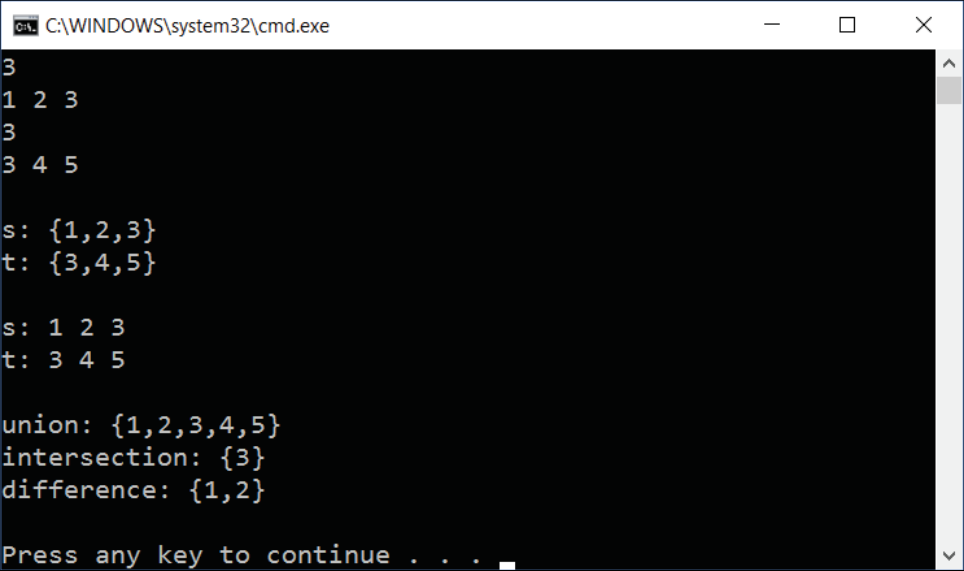
\includegraphics[width=0.85\textwidth]{images/p102_i04.png}\end{center}

\section{高级搜索与排序}

前一节我们研究了线性搜索。本节我们来看二分搜索。二分搜索算法先在列表中点处查找该值，然后用列表的一半继续搜索。这样，由于每一次迭代都把列表一分为二，它的时间效率是 $O(\log_2 n)$。

\medskip\noindent{\ttfamily\bfseries Search.h}

\begin{codebox}
template <class ListType, class ValueType>
int binarySearch(const ValueType& value, const ListType& list) {
  ListType::Iterator* positionBuffer =
    new ListType::Iterator[list.size()];

  int index = 0;
  for (ListType::Iterator position = list.begin();
       position != list.end(); ++position) {
    positionBuffer[index++] = position;
  }

  int minIndex = 0, maxIndex = list.size() - 1;

  while (minIndex <= maxIndex) {
    int middleIndex = (maxIndex + minIndex) / 2;
    ListType::Iterator iterator = positionBuffer[middleIndex];
    const ValueType& middleValue = *iterator;

    if (value == middleValue) {
      return middleIndex;
    }
    else if (value < middleValue) {
      maxIndex = middleIndex - 1;
    }
    else {
      minIndex = middleIndex + 1;
    }
  }

  return -1;
}
\end{codebox}

\subsection{归并排序算法}

归并排序算法把列表分成两个大小相等的子列表，通过递归调用对子列表排序（所谓递归调用，就是一个方法或函数调用它自己），然后以类似于前面扩展版 Set 类的 merge 方法的方式把有序的子列表合并起来。

\medskip\noindent{\ttfamily\bfseries Sort.h}

\begin{codebox}
template <class ListType, class ValueType>
void mergeSort(ListType& list) {
  int size = list.size();

  if (size > 1) {
    int middle = list.size() / 2;
    ListType::Iterator iterator = list.begin();

    ListType leftList;
    for (int count = 0; count < middle; ++count) {
      leftList.add(*iterator);
      ++iterator;
    }

    ListType rightList;
    for (; iterator != list.end(); ++iterator) {
      rightList.add(*iterator);
    }

    mergeSort<ListType, ValueType>(leftList);
    mergeSort<ListType, ValueType>(rightList);

    ListType resultList;
    merge<ListType, ValueType>(leftList, rightList, resultList);
    list = resultList;
  }
}
\end{codebox}

本节的 merge 方法复用了本章前面扩展版 Set 类中 merge 的思路：

\begin{codebox}
template <class ListType, class ValueType>
void merge(ListType& leftList, ListType& rightList,
           ListType& result) {
  ListType::Iterator leftPosition = leftList.begin();
  ListType::Iterator rightPosition = rightList.begin();

  while ((leftPosition != leftList.end()) &&
         (rightPosition != rightList.end())) {
    if (*leftPosition < *rightPosition) {
      result.add(*leftPosition);
      ++leftPosition;
    }
    else {
      result.add(*rightPosition);
      ++rightPosition;
    }
  }

  while (leftPosition != leftList.end()) {
    result.add(*leftPosition);
    ++leftPosition;
  }

  while (rightPosition != rightList.end()) {
    result.add(*rightPosition);
    ++rightPosition;
  }
}
\end{codebox}

\subsection{快速排序算法}

快速排序算法先选出第一个值（称为枢值，pivot value），然后把所有小于枢值的值放入较小的子列表，把所有大于或等于枢值的值放入较大的子列表。随后通过递归调用对这两个列表排序，最后只需把它们拼接在一起。我们来看下面的例子：

\begin{codebox}
template <class ListType, class ValueType>
void quickSort(ListType& list) {
  if (list.size() > 1) {
    ListType smaller, larger;
    ValueType pivotValue = *list.begin();

    ListType::Iterator position = list.begin();
    ++position;

    for (; position != list.end(); ++position) {
      if (*position < pivotValue) {
        smaller.add(*position);
      }
      else {
        larger.add(*position);
      }
    }

    quickSort<ListType, ValueType>(smaller);
    quickSort<ListType, ValueType>(larger);

    list = smaller;
    list.add(pivotValue);
    list.add(larger);
  }
}
\end{codebox}

归并排序是平衡的：它总是把列表分成相等的两部分并对它们排序。算法必须遍历列表一次才能把列表分成两个子列表，然后再对子列表排序。给定一个值列表，它必须遍历其 $n$ 个值，并把列表分割 $\log_2 n$ 次。因此，归并排序的时间效率为 $O(n \log_2 n)$。

而快速排序算法在最坏情况下（列表已经有序时）并不比插入排序、选择排序或冒泡排序好：同样是 $O(n^2)$。不过，它在平均情况下是很快的。

\section{小结}

本章我们为抽象数据类型列表和集合创建了类。列表是一种有头有尾的有序结构，而集合是一种无序结构。

我们先从相当简单的版本入手：列表带有独立的单元格类和迭代器类。接着我们创建了更高级的版本，使用了模板和运算符重载，并把单元格类和迭代器类放进了列表类内部。最后，我们引入了重载的引用方法。

同样地，我们先创建了一个相当简单、低效的集合类版本，然后创建了使用模板和运算符重载的更高级版本；在这个版本中，我们把值按顺序存放，以便更高效地执行并集、交集和差集运算。

此外，我们还实现了线性搜索和二分搜索算法。线性搜索可用于任何无序序列，但效率较低；二分搜索效率更高，但只能用于有序序列。

最后，我们研究了排序算法。我们先从简单但相当低效的插入排序、选择排序和冒泡排序入手，接着继续研究更高级、更高效的归并排序和快速排序算法。

下一章我们将开始构建一个图书馆管理系统。